\documentclass[12pt]{report}
\usepackage{amscd,amsthm,amsmath,amstext,amssymb,mathrsfs}
\usepackage{epsfig,longtable,verbatim,graphicx,multirow,array,wasysym,esint,hyperref,kotex,color}
\usepackage[T1]{fontenc}
\usepackage[sort&compress,square,numbers]{natbib}

\numberwithin{figure}{chapter}
\theoremstyle{plain}
\newtheorem{theorem}{\protect\theoremname}[chapter]
\theoremstyle{definition}
\newtheorem{definition}[theorem]{\protect\definitionname}
\theoremstyle{corollary}
\newtheorem{corollary}[theorem]{\protect\corollaryname}
  \theoremstyle{definition}
  \newtheorem{rem}[theorem]{\protect\remarkname}
  \theoremstyle{plain}
  \newtheorem{proposition}[theorem]{\protect\propositionname}
\theoremstyle{definition}
\newtheorem{claim}[theorem]{\protect\examplename}
  \theoremstyle{plain}
  \newtheorem{lemma}[theorem]{\protect\lemmaname}
\newtheorem{assumption}[theorem]{Assumption}

\renewcommand{\labelenumi}{(\roman{enumi})}

\makeatother

  \providecommand{\lemmaname}{Lemma}
  \providecommand{\propositionname}{Proposition}
  \providecommand{\remarkname}{Remark}
\providecommand{\theoremname}{Theorem}
\providecommand{\examplename}{Claim}
\providecommand{\definitionname}{Definition}
\providecommand{\corollaryname}{Corollary}

\newtheorem{question}{Question}

\newcommand\aint{-\hspace{-0.44cm}\int}
\renewcommand{\theequation}{\thesection.\arabic{equation}}

%% preamble part by ksj
\usepackage[onehalfspacing]{setspace}
\usepackage{booktabs,enumitem}
\newcommand\bs[1]{\ensuremath{\boldsymbol{#1}}}
\newcommand\bx{\ensuremath{\boldsymbol x}}
\newcommand\by{\ensuremath{\boldsymbol y}}
\newcommand\bb{\ensuremath{\boldsymbol b}}
\newcommand\bv{\ensuremath{\boldsymbol v}}
\newcommand\lip{\ensuremath{\text{Lip}}}

\begin{document}
\title{\textbf{Lipschitz Constants of Functions of Neural Networks}}
\author{\\\textbf{Sunjoong Kim}\\}
\setcounter{tocdepth}{1}
\date{}
 \maketitle{}

%\newpage
\tableofcontents
%\listoffigures

\newpage
\begin{abstract}

\end{abstract}
\newpage
\setcounter{page}{1} \setcounter{section}{0}


%%%
\chapter{Introduction}

Deep neural networks have made many advances including computer vision, language modeling, machine translation and text and picture generating.
Still, one of the difficulties in applying deep learning algorithms to reality is that the algorithm often lacks its robustness.
As an example, Szegedy et al. (2014) have found that a small perturbation of an input for true image may cause the classifier to misclasssify the image as false image.

To overcome the instabiltiy of training and to enhance robustness of generating models such as GANs, M. Arjovsky et al. (2017) proposed Wasserstein distance between distributions and restrict their attention to 1-Lipschitz function to the critic.
As this example suggest, the Lipschitz constant can be a good metric to access the robustness of the algorithm.

The Lipschitz constant of a function measures the sensitiveness or the robustness, or the rate of changes of the function.
In chapter 2, we define the optimal Lipschitz constant of the functions between euclidean spaces and explore the computation of this optimal constant for various functions including linear maps, affine maps and compositions of functions.
However, if the function becomes more complex, it is difficult or almost impossible to calculate the optimal constant.
So, we propose the algorithms to estimate the constant, using the Rademacher's theorem.

%%%
\chapter{Lipschitz Constants of Functions Between Euclidean Spaces}

%%
\section{Lipschitz Constants}
% Definition : A Liptschitz constant (LC) and The optimal Lipschitz constant(OLC), extension to the metric space functions
%Let \(f:\mathbb R^n\to\mathbb R^m\) be a function.
For vectors \(\bx=[x_1\:\:\cdots\:\:x_n]^T\) and \(\by=[y_1\:\:\cdots\:\:y_m]^T\) in Euclidean spaces \(\mathbb R^n\) and \(\mathbb R^m\), respectively, \(||\bx||\) and \(||\by||\) are the usual standard norms of \bx{} and \by{} defined by
\begin{equation}\label{eq:euclidean_norm}
||x||=\sqrt{{x_1}^2+\cdots+{x_n}^2},\quad ||y||=\sqrt{{y_1}^2+\cdots+{y_m}^2}.
\end{equation}

\begin{definition}\label{LC}
A function \(f:\mathbb R^n\to\mathbb R^m\) is called \emph{Lipschitz continuous} if there is a nonnegative real number \(c\) such that
\begin{equation}\label{eq:LC1}
||f(\bx)-f(\by)||\le c||\bx-\by||\qquad(\bx,\by\in\mathbb R^n)
\end{equation}
The infimum of \(c\) which satisfies \eqref{eq:LC1} is called the \emph{Lipschitz constant} of \(f\) and is denoted by \(\lip(f)\).
%If \(\lip(f)\) exists as a nonnegative real number, \(f\) is called a Lipschitz continuous function.
\end{definition}

% The equality of inf-def and sup-def
This definition can also be extended to functions from a metric space to another metric space if we replace the norms by the distances.
It is useful to know that there is an equivalent definition ;
\begin{equation}\label{eq:LC2}
\lip(f)=\sup_{\bx\neq\by}\frac{||f(\bx)-f(\by)||}{||\bx-\by||}
\end{equation}
To prove the equality, let
\begin{equation}\label{eq:equivalent_def}
\begin{aligned}
L_1&=\inf\{c\ge0:||f(\bx)-f(\by)||\le c||\bx-\by||,\quad\bx,\by\in\mathbb R^n\}\\
L_2&=\sup\left\{\frac{||f(\bx)-f(\by)||}{||\bx-\by||}:\bx,\by\in\mathbb R^n,\bx\neq\by\right\}.
\end{aligned}
\end{equation}
Let \(\mathcal L_1\) and \(\mathcal L_2\) be two the sets in the definition of \(L_1\) and \(L_2\), respectively.
Then, \(\mathcal L_2\subset\mathcal L_1\) since
\[\mathcal L_2=\{c\ge0:||f(\bx)-f(\by)||=c||\bx-\by||,\quad\bx,\by\in\mathbb R^n,\bx\neq\by\},\]
and it follows that \(L_1\le L_2\).
%Pick \(c\in\mathcal L_2\).
%Then, \(c\in\mathcal L_1\) and it follows that \(L_1=\inf\mathcal L_1\le c\).
%Since \(c\in\mathcal L_2\) was arbitrary, we can take supremum for all \(c\in\mathcal L_2\) to conclude that \(L_1\le L_2\).
Pick \(c\in\mathcal L_1\).
Then, \(||f(\bx)-f(\by)||\le c||\bx-\by||\) for all \(\bx\) and \(\by\) in \(\mathbb R^n\).
Assuming \(\bx\neq \by\), we have
\[
\frac{||f(\bx)-f(\by)||}{||\bx-\by||}\le c.
\]
Taking supremum for all \bx{} and \by{} (\(\bx\neq\by\)), we have \(L_2\le c.\) and taking infimum for all \(c\le\mathcal L_1\) yields \(L_2\le L_1\).

% inf = min
The optimal Lipschitz constant \(\lip(f)\) is not only the infimum, but also the minimum of \(L\) satisfying \eqref{eq:LC1}.
To show this, it suffices to show that \(\lip(f)\in\mathcal L_1\), or that \(c=\lip(f)\) satisfies the condition.
Let \(\bx,\:\by\in\mathbb R^n\).
If \(\bx=\by\), then \eqref{eq:LC1} holds trivially.
Assuming \(\bx\neq\by\), we have
\[
\frac{||f(\bx)-f(\by)||}{||\bx-\by||}\le\lip(f)
\]
because of the second definition \eqref{eq:LC2} of \(\lip(f)\).
Multiplying both sides by \(||\bx-\by||\), we can conclude that \(c=\lip(f)\) satisfies the condition \eqref{eq:LC1}.
% sup = max도 증명하면 좋겠는데, 어떻게 해야 할 지 모르겠다.
% f가 linear map인 경우에는 conrad의 방법을 사용하면 된다.
% conrad의 방법을 여기에 쓰자니, 가능은 할 것 같은데 말이 너무 길어지는 것 같다.

% lip=0 iff constant function
Note also that \(\lip(f)=0\) if and only if \(f\) is a constant function.
Suppose that \(f\) is a constant function.
Then, the condition \eqref{eq:LC1} holds vacuously and \(\mathcal L_1=[0,\infty)\) ; \(\lip(f)=0\).
Suppose, on the contrary, that \(\lip(f)=0\).
Pick \(\bx,\by\in\mathbb R^n\).
Since \(0\in\mathcal L_1\), we have \(||f(\bx)-f(\by)||=0\).
Thus, \(f(\bx)=f(\by)\) and \(f\) is a constant function.
% Finding OLC is NP-hard [1]

%%
\section{Real-valued Functions of a Real Variable}
% Average rate of change
% differentiable (almost) everywhere → mean value theorem
% sigmoid, hyperbolic tangent, ReLU

For univariate real function \(f:\mathbb R\to\mathbb R\), the above condition \eqref{eq:LC1} is equivalent to saying that the average rate of change is upper bounded by \(c\);
\begin{equation}\label{eq:LC_average_rate_of_change}
\left|\frac{f(x)-f(y)}{x-y}\right|\le c.
\end{equation}
If \(f\) is diffrentiable everywhere in the domain, the mean value theorem guarantees that this is equivalent to 
\begin{equation}\label{eq:LC_univariate1}
|f'(x)|\le c
\end{equation}
for every \(x\in\mathbb R\).
Moreover, \(\lip(f)\) is the least nonnegative number \(c\) satisfying the condition \eqref{eq:LC_univariate1} for all \(x\) and we can express \(\lip f\) in its exact form ; 
\begin{equation}\label{eq:LC_univariate2}
\lip (f) = \sup_{x\in\mathbb R}|f'(x)|
\end{equation}

In this sense, we can easily evaluate the optimal Lipschitz constant of the sigmoid function
\begin{equation}\label{eq:sigmoid}
\sigma(x)=\frac1{1+e^{-x}}
\end{equation}
and the hyperbolic tangent function
\begin{equation}\label{eq:tanh}
\tanh(x)=\frac{e^x-e^{-x}}{e^x+e^{-x}}.
\end{equation}
Since \(0<\sigma(x)<1\) and \(\sigma'(x)=\sigma(x)\left(1-\sigma(x)\right)\), we have \(\sigma'(x)<\frac14\) so that
\begin{equation}\label{eq:sigmoid_LC}
\lip(\sigma)=\frac14.
\end{equation}
Since \(\tanh(x)=2\sigma(2x)-1\), we have
\[\tanh'(x)=4\sigma'(2x)<1\]
and
\begin{equation}\label{eq:tanh_LC}
\lip(\tanh)=1.
\end{equation}

The \text{ReLU} function
\begin{equation}\label{eq:ReLU}
\text{ReLU}(x)=\max\{0,x\}
\end{equation}
 is not differentiable everywhere, but we can use \eqref{eq:LC_average_rate_of_change} to conclude
\begin{equation}\label{eq:ReLU_LC}
\lip(\text{ReLU})=1.
\end{equation}
%Although not being differentiable, the case of rectified linear unit \(\text{ReLu}(x)=\max\{0,x\}\) can also be easily evaluated to be \(1\).
Here is a list of the optimal Lipschitz constants of univariate activation functions, frequently used in machine learning and deep learning.
 
\renewcommand\arraystretch{1.5}
\begin{table}[ht]
\centering
\caption{The optimal Lipschitz constants of univariate activation functions.
\(\alpha=0.1\) for Leaky ReLU and \(\alpha=1\) for ELU.}
\begin{tabular}[t]{llc}
\toprule
Activation Functions	&Formula									& $\lip(f)$\\
\midrule
Sigmoid				&$\sigma(x)=\frac1{1+e^{-x}}$				&$\frac14$\\
Hyperbolic tangent	&$\tanh(x)=\frac{e^x-e^{-x}}{e^x+e^{-x}}$	&1\\
Rectified Linear Unit	&$\text{ReLU}(x)=\max\{0,x\}$			&1\\
Leaky ReLU			&$\text{LReLU}(x)=\max\{\alpha x,x\}$	&1\\
Exponential Linear Unit&$\text{ELU}(x)=
\begin{cases}x&(x\ge0)\\\alpha(e^x-1)&(x<0)\end{cases}$	&1\\
Softplus			&$f(x)=\frac1\beta\log(1+e^{\beta x})$	&$1$\\
Gaussian			&$g(x)=e^{-x^2}$								&$\sqrt{\frac2e}$\\
\bottomrule
\end{tabular}
\end{table}

In the definition of \(\lip(f)\) in \eqref{eq:LC2}, we can't replace the supremum by the maximum.
Consider a function ; \(f(x)=\ln(1+e^x)\).
This function is called the softplus activation function and is an antiderivative of the sigmoid function.
It is a monotonically increasing function whose derivative is also increasing, with an assymptote \(y=x\).
Thus, \(\lip(f)=1\), but no \(x\) and \(y\) satisfy the equality \(\frac{f(x)-f(y)}{x-y}=1\).

%%
\section{Linear Functions}
% Operator norms of matrices matches the notion of OLC

%
\subsection{Operator Norms \(||W||\)}

Consider a linear function \(f(\bx)=W\bx\) for some \(m\times n\) matrix \(W\).
Because of the linearity, the condition \eqref{eq:LC1} reduces to
\begin{equation}\label{eq:linear_LC}
||W\bx||\le c||\bx||.\qquad(\bx\in\mathbb R^n)
\end{equation}

The smallest \(c\) which satisfies \eqref{eq:linear_LC} is called \emph{the operator norm of \(W\)} and denoted by \(||W||\).
Thus, the optimal Lipstchitz constant of \(f\) equals the operator norm of \(W\) ; \(||W||=\lip(f)\).
The definitions of the forms \eqref{eq:equivalent_def} are as follows;
\begin{equation}\label{eq:linear_equivalent_def}\begin{aligned}
||W||
&=\inf\left\{c\ge0\::\: ||W\bx||\le c||\bx||\right\}\\
&=\sup\left\{\frac{||W\bx||}{||\bx||}\;:\;\bx\in\mathbb R^n,\:\bx\neq\bs0\right\}
\end{aligned}\end{equation}
If we modify the second definition of \eqref{eq:linear_equivalent_def} to
\begin{equation}\label{eq:linear_equivalent_def_2}
||W||=\sup\left\{||W\bx||:||\bx||=1\right\},
\end{equation}
we can easily verify that the supremum is actually the maximum in this case.
Because the set \(\{\bx:||\bx||=1\}\) is a compact subset of \(\mathbb R^m\) and the map \(\bx\mapsto||W\bx||\) is continuous, the set in \eqref{eq:linear_equivalent_def_2} has its maximum.

The operator norm is indeed a norm of a vector space ;
\begin{proposition}\label{prop:operator_norm_1}
The operator \(||\cdot||:W\mapsto||W||\) satisfies the following three properties.
Thus, the set \(\mathcal M_{m,n}(\mathbb R)\) of all \(m\) by \(n\) real matrices is a normed vector space with respect to this norm ;
\begin{enumerate}[label=(\alph*)]
\item
\(||W||\ge0\) for all \(W\in\mathcal M_{m,n}(\mathbb R)\) ; \(||W||=0\) if and only if \(W=0\).
\item
\(||kW||=|k|\cdot||W||\) for all \(W\in\mathcal M_{m,n}(\mathbb R)\) and \(k\in\mathbb R\).
\item
\(||W+V||\le||W||+||V||\) for all \(W,V\in\mathcal M_{m,n}(\mathbb R)\).
\end{enumerate}
\end{proposition}
For (a), that \(||W||\ge0\) is obvious.
If \(||W||=0\), then \(||W\bx||\le 0||\bx||=0\) for all \(\bx\in\mathbb R^n\).
It follows that \(W\bx=0\) for all \(\bx\in\mathbb R^n\), by the definition of vector norm, for which \(W=0\)
Suppose, on the other hand, that \(W=0\). Then \(W\bx=0\) for all \(x\in\mathbb R^n\).
Thus, \(c=0\) is the minimal value satisfying \eqref{eq:linear_LC}.
To prove (b), we have
\begin{align*}
||kW||
&=\inf\left\{c:||kWx||\le c||x||\right\}\\
&=\inf\left\{c:|k|\cdot||Wx||\le c||x||\right\}\\
&=\inf\left\{c:||Wx||\le\frac{c}{|k|}||x||\right\}\\
&=\inf\left\{|k|b:||Wx||\le b||x||\right\}\\
&=|k|\inf\left\{b:||Wx||\le b||x||\right\}\\
&=|k|\cdot||W||.
\end{align*}
Now, consider (c).
For any \(\bx\in\mathbb R^n\), we have
\begin{align*}
||(W+V)\bx||
&=||W\bx+V\bx||\le||W\bx||+||V\bx||\\
&\le||W||\:||\bx||+||V||\:||\bx||=(||W||+||V||)||\bx||
\end{align*}
By the minimality of \(||W+V||\), we have \(||W+V||\le||W||+||V||\).

An analogue of (c) also holds for multiplication;
if \(W\in\mathcal M_{m,n}(\mathbb R)\) and \(V\in\mathcal M_{n,k}(\mathbb R)\), then
\begin{equation}\label{eq:multiplicative_inequality}
||WV||\le||W||\:||V||.
\end{equation}
This is because of the inequality
\[||(WV)\bx||=||W(V\bx)||\le||W||\:||V\bx||\le||W|\:||V||\:||\bx||\]
and the minimality of \(||WV||\).

%
\subsection{Evaluation of \(||W||\) for square matrices}

First, consider the case when \(W\) is a square matrix so that \(f:\mathbb R^n\to\mathbb R^n\).
Let \(\lambda_1\), \(\cdots\), \(\lambda_n\) be (possibly repeated) eigenvalues of \(W\) and let \(\tilde\lambda=\max\{|\lambda_i|\::\:i=1,\cdots,n\}\).
Then, the following inequality holds in general ;
\begin{equation}\label{eq:square_matrix_equation_1}
\tilde\lambda\le||W||.
\end{equation}
For a proof, pick an eigenvalue \(\lambda_i\) and the corresponding eigenvector \(\bx_i\) which is nonzero.
Since \(W\bx_i=\lambda_i\bx_i\),
Then, we have \(||W\bx_i||=|\lambda_i|\:||\bx_i||\) and
\[|\lambda_i|=\frac{||W\bx_i||}{||\bx_i||}\le||W||.\]
Taking the maximum over \(i\), we have the desired inequality.
The above inequality \eqref{eq:square_matrix_equation_1} becomes equality when \(W\) is symmetric.

Suppose that \(W\) is real symmetric.
Then, \(W\) is orthogonally diagonalizable in the sense that, there exists an orthogonal matrix
\[V=[\bv_1\quad \cdots \quad \bv_n],\]
%which is orthogonal (and thus \(\{\bv_1,\cdots,\bv_n\}\) is orthonormal.)
such that
\[W=V\Lambda V^T,\]
where \(\Lambda=\text{diag}\{\lambda_1,\cdots,\lambda_n\}\) and \(\lambda_i\) is an eigenvalue of \(W\) with the corresponding eigenvector \(\bv_i\).
Note that \(\{\bv_1,\cdots,\bv_n\}\) forms an orthonormal basis for \(\mathbb R^n\).
For any \(\bx\in\mathbb R^n\), there exist real numbers \(c_1\), \(\cdots\), \(c_n\) such that \(\bx=c_1\bv_1+\cdots+c_n\bv_n\).
Since
\begin{align*}
W\bx
&=c_1W\bv_1+\cdots+c_nW\bv_n\\
&=c_1\lambda_1\bv_1+\cdots+c_n\lambda_n\bv_n,
\end{align*}
we have
\begin{align*}
||W\bx||^2
&=||c_1W\bv_1+\cdots+c_nW\bv_n||^2\\
&=|c_1\lambda_1|^2||\bv_1||^2+\cdots+|c_n\lambda_n|^2||\bv_n||^2\\
&={c_1}^2{\lambda_1}^2+\cdots+{c_n}^2{\lambda_n}^2.
\end{align*}
Thus,
\[\frac{||W\bx||^2}{||\bx||^2}=\frac{{c_1}^2{\lambda_1}^2+\cdots+{c_n}^2{\lambda_n}^2}{{c_1}^2+\cdots+{c_n}^2}
\le{\tilde\lambda}^2,\]
for which \(||W\bx||/||\bx||\le\tilde\lambda\).
Therefore, we have the reverse inequality \(||W||\le\tilde\lambda\).

As examples consider the following matrices \(W_1\), \(W_2\), \(W_3\), \(W_4\), \(W_5\) defined by
\begin{gather*}
W_1=\begin{bmatrix}
1&0\\0&1
\end{bmatrix},\quad
W_2=\begin{bmatrix}
2&0\\0&3
\end{bmatrix},\quad
W_3=\begin{bmatrix}
4&2\\2&7
\end{bmatrix},\\
W_4=\begin{bmatrix}
1&3\\2&0
\end{bmatrix},\quad
W_5=\begin{bmatrix}
0&1\\0&0
\end{bmatrix}.\quad
\end{gather*}
\(W_1\) is the identity matrix and thus \(||W||=1\).
Indeed, the characteristic polyinomial of \(W_1\) is \((\lambda-1)^2=0\), \(\lambda_1=\lambda_2=1\) and thus the maximum absolute value of them is \(1\).
The matrix \(W_2\) stretches a given vector \(\bx\) twice in the x-axis direction and three times in the y-axis direction.
Thus, \(||W_2||\) should be \(3\).
Indeed, \(|W_2-\lambda I|=(\lambda-2)(\lambda-3)\) and \(\tilde\lambda=3\).
\(W_3\) is the last example that is symmetric ; \(|W_3-\lambda I|=(\lambda-3)(\lambda-8)\) and \(\tilde\lambda=8\).

\(W_4\) is not symmetric and we can't evaluate \(||W_4||\) for now.
Still, we have, \(\lambda_1=-2\), \(\lambda_2=3\) and \(||W_4||\ge3\) by \eqref{eq:square_matrix_equation_1}.
The reverse inequality is not valid since the eigenvectors \(x_1=[1\:\:-1]^T\) and \(x_2=[3\:\:2]^T\) are not perpendicular.
\(W_5\) is not symmetric either, but we can postulate that \(||W_5||=1\) since
\[
W_5\bx=
\begin{bmatrix}
0&1\\0&0
\end{bmatrix}
\begin{bmatrix}
x_1\\x_2
\end{bmatrix}
=
\begin{bmatrix}
x_2\\0
\end{bmatrix}
\]
and
\[
\frac{||W_5\bx||}{||\bx||}=\frac{|x_2|}{\sqrt{{x_1}^2+{x_2}^2}}\le 1.
\]
Since \(W_5\) has the only eigenvector \(0\), the inequality \eqref{eq:square_matrix_inequality_1} still holds.

Here is a short description of what we've done in this subsection.
\begin{lemma}\label{lemm:evaluation_for_square_matrices}
Let \(W\in\mathcal M_n(\mathbb R)\) be a real symmetric matrix.
Then, the operator norm \(||W||\) is the maximal absolute eigenvalue of \(W\).
\end{lemma}

%
\subsection{Evaluation of \(||W||\) for rectangular matrices}
Almost all matrices that we encounter in machine learning problem are neither square matrices, nor are they symmetric matrices.
But, we can always calculate the Lipschitz constant or the operator norm of any rectangular matrices.
Aside from the properties listed in the Proposition \ref{prop:operator_norm_1}, there is a useful criteria that help find the optimal Lipschitz constant of any rectangular matrix.

\begin{theorem}\label{theo:evaluation_for_rectangular_matrices}
Let \(W\in\mathcal M_{m,n}(\mathbb R)\) be an \(m\) by \(n\) real matrix.
Then
\begin{equation}\label{eq:evaluation_of_operator_norm_for_rectangular_matrix}
||W||=\sqrt{||W^TW||}.
\end{equation}
\end{theorem}

Note that the norm on the left hand side is the operator norm on \(\mathcal M_{m,n}(\mathbb R)\) and the norm on the right hands side is the operator norm on \(\mathcal M_n(\mathbb R)\).
Note also that the matrix \(W^TW\) is symmetric in that \((W^TW)^T=W^T(W^T)^T=W^TW\) and we are always able to calculate the norm of \(||W^TW||\) by making use of the lemma \ref{lemm:evaluation_for_square_matrices}.

Before the proof of \eqref{eq:evaluation_of_operator_norm_for_rectangular_matrix}, we illustrate elementary properties of the operator norm of matrices.
The euclidean norm \(||\bx||\) of a vector \(\bx\in\mathbb R^n\) in \eqref{eq:euclidean_norm} can also be defined by means of the inner product on \(\mathbb R^n\);
\begin{equation}\label{eq:euclidean norm_2}
||\bx||=\sqrt{\langle \bx,\bx\rangle}.
\end{equation}
The inner product \(\langle \bx,\by\rangle=\bx^T\by\) has the following properties and we omit the proofs of them.
\begin{gather*}
\langle \bx,W\by\rangle=\langle W^T\bx,\by\rangle,\\
\langle k\bx,\by\rangle=k\langle \bx,\by\rangle,\\
|\langle\bx,\by\rangle|\le||\bx||\:||\by||.
\end{gather*}

Now we are ready for the proof of \eqref{eq:evaluation_of_operator_norm_for_rectangular_matrix}.
If \(W=0\), then the equation \eqref{eq:evaluation_of_operator_norm_for_rectangular_matrix} holds trivially.
Suppose that \(W\neq0\).
Let \(\bx\in\mathbb R^n\).
Then
\begin{align*}
||W\bx||^2
&=\langle W\bx,W\bx\rangle\\
&=\langle W^TW\bx,\bx\rangle\\
&\le||W^TW\bx||\:||\bx||\\
&\le||W^TW||\:||\bx||^2,
\end{align*}
and thus
\[||W\bx||\le\sqrt{||W^TW||}\:||\bx||.\]
for all \(\bx\in\mathbb R^n\).
By the minimality of \(||W||\), we have
\[||W||\le\sqrt{||W^TW||}\]
Squaring both sides and making use of \eqref{eq:multiplicative_inequality} yield
\begin{equation}\label{eq:half_inequality}
||W||^2=||W^TW||\le||W^T||\:||W||.
\end{equation}
Since \(||W||\neq0\), we have
\[||W||\le||W^T||.\]
Substituting \(W\) by its transpose, we get the reverse inequality.
Therefore,
\begin{equation}\label{eq:norm_and_transpose}
||W||=||W^T||.
\end{equation}
By \eqref{eq:norm_and_transpose}, the equation \eqref{eq:half_inequality} reduces to
\[||W||^2=||W^TW||,\]
and this proves \eqref{eq:evaluation_of_operator_norm_for_rectangular_matrix}.

For example, we can evaluate the operator norm of \(W_4\) and \(W_5\) in the previous subsection.
We have
\[{W_4}^TW_4=\begin{bmatrix}1&3\\2&0\end{bmatrix},\quad{W_5}^TW_5=\begin{bmatrix}0&0\\0&1\end{bmatrix}.\]
\({W_4}^TW_4\) has its eigenvalues \(7\pm\sqrt{13}\), thus \(||W_4||=\sqrt{7+\sqrt{13}}\).
And \({W_5}^TW_5\) has eigenvalues \(0\) and \(1\) ; \(||W_5||=\sqrt1=1\) as expected.
As a rectangular matrix, we may think of
\[W_6=\begin{bmatrix}1&0\\2&1\\0&1\end{bmatrix}.\]
Since
\[{W_6}^TW_6=\begin{bmatrix}5&2\\2&2\end{bmatrix},\]
\(\lambda=1,6\) and \(||W_6||=\sqrt6\).

%%
\section{Affine Functions}
An affine function 
\begin{equation}\label{eq:affine}
f(\bx)=W\bx+\bb
\end{equation}
has the same optimal Liptschitz constant as that of its linear part ; 
\begin{equation}\label{eq:affine_LC}
\lip(f)=||W||
\end{equation}
This is because the condition \eqref{eq:LC1} 
\[
||f(\bx)-f(\by)||\le c||\bx-\by||
\]
applied to \eqref{eq:affine} becomes
\[
||W(\bx-\by)||\le c||\bx-\by||.
\]

%%
\section{Elementwise Application of Nonlinear Functions}
Let \(f:\mathbb R\to\mathbb R\) be any function and let \(F:\mathbb R^m\to\mathbb R^m\) be applying \(f\) to each element of the input \(\bx = [x_1\:\cdots\:x_m]^T\) :
\begin{equation}\label{eq:elementwise}
F(\bx)=F\left(\begin{bmatrix}x_1\\\vdots\\x_m\end{bmatrix}\right)=
\begin{bmatrix}f(x_1)\\\vdots\\f(x_m)\end{bmatrix}.
\end{equation}
If \(f\) is a Liptschitz continuous function with its optimal constant \(L\).
Then,
\begin{align*}
||F(\bx)-F(\by)||^2
&=\left|\left|\begin{bmatrix}f(x_1)-f(y_1)\\\vdots\\f(x_m)-f(y_m)\end{bmatrix}\right|\right|^2
=\sum_{i=1}^m|f(x_i)-f(y_i)|^2\\
&\le\sum_{i=1}^mL^2|x_i-y_i|^2=L^2||\bx-\by||^2,
\end{align*}
for which
\[||F(\bx)-F(\by)||\le L||\bx-\by||.\]
Thus, \(\lip(F)\) is upper bounded by \(L=\lip(f)\) ;
\begin{equation}\label{eq:elementwise_LC}
\lip(F)\le\lip(f).
\end{equation}

%%
\section{Composites of Functions}
Let \(f:\mathbb R^n\to\mathbb R^m\) and \(g:\mathbb R^m\to\mathbb R^k\) be Lipstchitz continuous functions.
Then, the composite function \(g\circ f\) is also Lipstchitz continuous and the optimal constant is bounded by the product of those of \(f\) and \(g\) ; 
\begin{equation}\label{eq:composite_1}
\lip(g\circ f)\le\lip(f)\lip(g)
\end{equation}

This is readily proved by the following reason.
Let \(L\) and \(M\) be the optimal Lipschitz constants for \(f\) and \(g\) respectively.
Then, for all \(\bx,\by\in\mathbb R^n\),
\begin{align*}
||(g\circ f)(\bx)-(g\circ f)(\by)||
&=||g(f(\bx))-g(f(\by))||\\
&\le M||f(\bx)-f(\by)||\\
&\le LM||\bx-\by||.
\end{align*}
By the minimality of \(\lip(g\circ f)\), we have \eqref{eq:composite_1}.

Note that \eqref{eq:multiplicative_inequality} is a specific case of \eqref{eq:composite_1}.
Here, the inequality can be strict.
As an example, \(||W_2||\:||W_4||=3\times\sqrt{7+\sqrt{13}}>\sqrt{1+\sqrt{37}}=||W_2W_4||\).
Note also that \eqref{eq:composite_1} can be generalized further, to the case when the composition involoves several functions.
That is, if \(f_i:\mathbb R^{n_{i-1}}\to\mathbb R^{n_i}\) are  functions between euclidean spaces, with its optimal Lipschitz constant \(L_i\), for \(i=1,2,\cdots,p\), the composite
\[f_p\circ\cdots\circ f_1:\mathbb R^{n_1}\to\mathbb R^{n_{p+1}}\]
is Lipschitz constinuous and
\begin{equation}\label{eq:composite_2}
\lip(f_p\circ\cdots\circ f_1)\le\prod_{i=1}^kL_i.
\end{equation}

%%%
\chapter{Lipschitz Constants of Neural Networks}

Now we turn to the problem of finding the optimal Lischitz constant of various architectures frequently appearing in machine learning and deep learning.
%In this chapter, we use the term "Lipschitz constant of a function" to stand for the optimal Lipschitz constant of a function.

For locally Lipschitz function, it is possible to express the Lipschitz constant of \(f\) in its exact form, as the Rademacher Theorem suggests.
But, it is not always easy or feasible to find the exact value of Lipschitz constant whenever the function \(f\) is given.
In fact, although the function is of simple form such as 2-layered MLP, the problem of evaluating the Lipschitz function is NP-hard.
Instead of struggling to find analytic solutions, we present a systematic algorithm for each architectuare of neural network.

%%
\section{Rademacher Theorem}
Here is a theorem that can be applied to all Lipschitz functions between euclidean spaces.
The Lipschitz condition that we impose is not the global one \eqref{eq:LC1} ; it only need to be locally Lipschitz.
It has two conclusions : the differentiability (a.e.) and the formula for the optimal constant.

\begin{theorem}\label{theo:Rademacher}
Let \(f:\mathbb R^n\to\mathbb R^m\) be a locally Lipschitz function.
Then,
\(f\) is differentiable almost everywhere, and
\end{theorem}
\begin{equation}
\lip(f) = \sup_{\bx\in\mathbb R^n}||D_{\bx}(f)||
\end{equation}

The first statement --- differentiability --- is usually refered to the main conclusion of this theorem.
But the proof of it is so lengthy that we omit the proof here.
As for one-dimensional case, many of the textbooks of analysis including \cite{WR} covered this issue.
In the process, concepts like absolute continuity, Radon-Nykodym theorem, total variation are involved.

The second statement, or the optimal Lipschitz constant is the one that we can use for our purpose.
Note first that, \(D_{\bx}f\) is the Jacobian matrix of \(f\) or a matrix \(A\) satisfying
\[\lim_{\by\to\bx}\frac{||f(\by)-f(\bx)-A(\by-\bx)||}{||\by-\bx||}=0,\]
and that \(||D_{\bx}(f)||\) is nothing but the operator norm we've defined in the previous chapter.

%%
\section{AutoLip : Upperbounding the Lipschitz constant by an algorithmic method}

Consider, for example, a univariate function \(f_\omega\) with a parameter \(\omega\) defined by
\[f_\omega(x) = \frac1{1+e^{-x}}+\left|2x+\omega\cos x\right|.\]
In order to construct a systematic way to estimate the constant and to make use of automatic differentiation in implementing the backpropagation by Tensorflow or Pytorch, we think of a computation graph for \(f_\omega\). (Figure \ref{computational_graph})

\begin{figure}
\centering
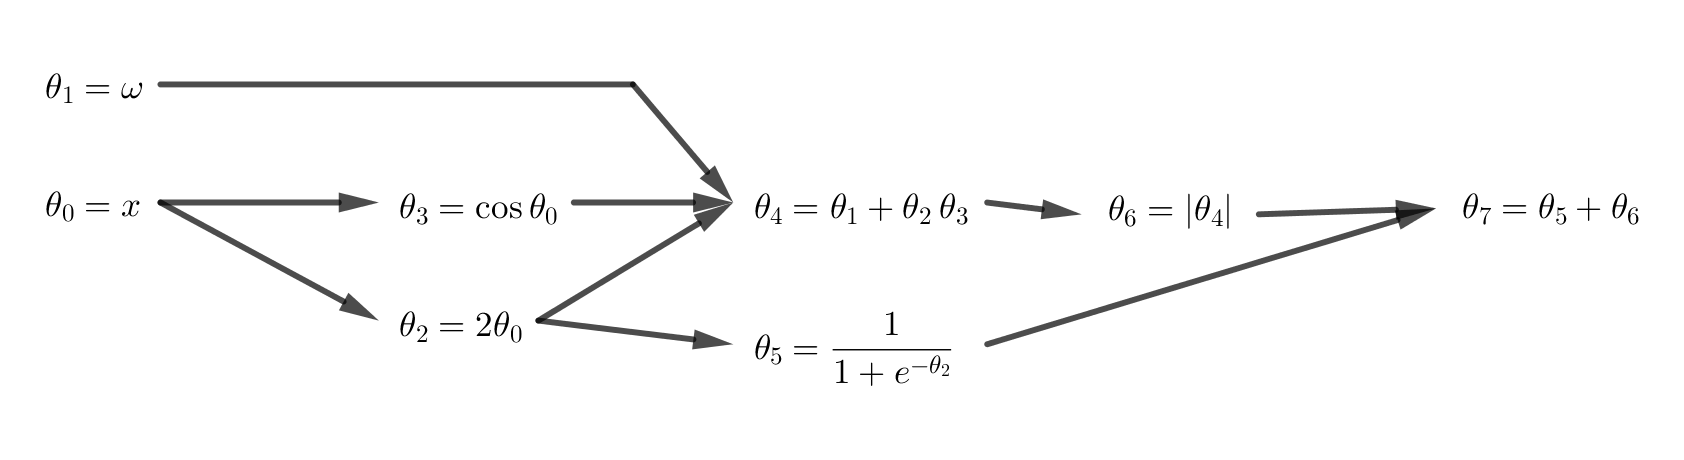
\includegraphics[width=\textwidth]{computation_graph}
\caption{A computational graph for the function \(f_\omega(x)=\frac1{1+e^{-x}}+\left|2x+\omega\cos x\right|.\)}
\label{computational_graph}
\end{figure}

%The derivative of \(f_\omega\), and the Lipschitz constant of it can be evaluated consecutively as follows.
Since, \(\theta_i\) is a function of \(\theta_0\), \(\theta_1\), \(\theta_2\), \(\cdots\), \(\theta_{i-1}\), the partial derivative \(\frac{\partial\theta_i}{\partial x}\) can be evaluated inductively as follows.

\begin{align*}
\frac{\partial\theta_1}{\partial x}&=0\\
\frac{\partial\theta_2}{\partial x}&
=\frac{\partial\theta_2}{\partial\theta_0}\frac{\partial\theta_0}{\partial x}
+\frac{\partial\theta_2}{\partial\theta_1}\frac{\partial\theta_1}{\partial x}
=\\
\frac{\partial\theta_3}{\partial x}&=\\
\frac{\partial\theta_4}{\partial x}&=\\
\frac{\partial\theta_5}{\partial x}&=\\
\frac{\partial\theta_6}{\partial x}&=\\
\frac{\partial\theta_7}{\partial x}&=
\end{align*}

%%
\section{AutoGrad}

%%%
\chapter{Conclusion}



\newpage



\newpage

\addcontentsline{toc}{chapter}{Bibliography}
\begin{thebibliography}{AA}
\bibitem {KS} Scaman, K. (2018, May 28). Lipschitz regularity of deep neural networks: analysis and. . . arXiv.org. Retrieved September 19, 2022, from https://arxiv.org/abs/1805.10965
\bibitem {CS-WZ} Christian Szegedy, Wojciech Zaremba, Ilya Sutskever, Joan Bruna, Dumitru Erhan, Ian Goodfellow, and Rob Fergus. Intriguing properties of neural networks.
In {\em Proceedings of the International Conference on Learning Representations (ICLR)}, 2014.
\bibitem {MA-SC} Martín Arjovsky, Soumith Chintala, and Léon Bottou.
Wasserstein generative adversarial networks.
In {\em Proceedings of the 34th International Conference on Machine Learning, ICML,} pages 214–223, 2017.
\bibitem {IG-YB} Ian Goodfellow, Yoshua Bengio, and Aaron Courville.
{\em Deep Learning.}
MIT Press, 2016.
\bibitem {FC} Francis H. Clarke. {\em On the Inverse function Theorem}, Pacific Journal of Mathematics, Vol 64, No. 1.
\bibitem {MJ-AD} Matt Jordan and Alexandros G. Dimakis {\em Exactly Computing the Local Lipschitz Constant of ReLUnetworks}
\bibitem {BA-DS} Bhowmick, Aritra \& D’Souza, Meenakshi \& Raghavan, G.. (2021). LipBaB: Computing Exact Lipschitz Constant of ReLU Networks. 10.1007/978-3-030-86380-7\_13. 
\bibitem {WR}  Rudin, Walter. {\em Real and Complex Analysis.} : McGraw-Hill Science/Engineering/Math, 1986.
\bibitem {HF} Herbert Federer. {\em Geometric measure theory.}
    Classics in Mathematics. Springer-Verlag Berlin Heidelberg, 1969.


\end{thebibliography}

%\addcontentsline{toc}{chapter}{Bibliography}
%
%\bibliographystyle{abbrv}
%\bibliography{reference.bib}
%
%



\end{document}

